\let\negmedspace\undefined
\let\negthickspace\undefined
\documentclass[journal]{IEEEtran}
\usepackage[a5paper, margin=10mm, onecolumn]{geometry}
%\usepackage{lmodern} % Ensure lmodern is loaded for pdflatex
\usepackage{tfrupee} % Include tfrupee package

\setlength{\headheight}{1cm} % Set the height of the header box
\setlength{\headsep}{0mm}     % Set the distance between the header box and the top of the text

\usepackage{gvv-book}
\usepackage{gvv}
\usepackage{cite}
\usepackage{amsmath,amssymb,amsfonts,amsthm}
\usepackage{algorithmic}
\usepackage{graphicx}
\usepackage{textcomp}
\usepackage{xcolor}
\usepackage{txfonts}
\usepackage{listings}
\usepackage{enumitem}
\usepackage{mathtools}
\usepackage{gensymb}
\usepackage{comment}
\usepackage[breaklinks=true]{hyperref}
\usepackage{tkz-euclide} 
\usepackage{listings}
\usepackage{tikz}
\usetikzlibrary{patterns}
% \usepackage{gvv}                                        
\def\inputGnumericTable{}                                 
\usepackage[latin1]{inputenc}                                
\usepackage{color}                                            
\usepackage{array}                                            
\usepackage{longtable}                                       
\usepackage{calc}                                             
\usepackage{multirow}                                         
\usepackage{hhline}                                           
\usepackage{ifthen}                                           
\usepackage{lscape}
\usepackage{multicol}
\begin{document}

\bibliographystyle{IEEEtran}
\vspace{3cm}

\title{ME : Mechanical Engineering}
\author{AI24BTECH11022 - Pabbuleti Venkata Charan Teja}
\maketitle

\renewcommand{\thefigure}{\theenumi}
\renewcommand{\thetable}{\theenumi}


\begin{enumerate}
\item He is known for his unscrupulous ways. He always sheds \rule{1cm}{0.15mm} tears to deceive people. \hfill(2020)
\begin{multicols}{2}
\begin{enumerate}
\item fox's
\item crocodile's
\item crocodile
\item fox
\end{enumerate}
\end{multicols}


\item Jofra Archer, the England fast bowler, is \rule{1cm}{0.15mm} than accurate. \hfill(2020)
\begin{multicols}{2}
\begin{enumerate}
\item more fast
\item faster
\item less fast
\item more faster
\end{enumerate}
\end{multicols}


\item Select the word that fits the analogy:

Build : Building :: Grow : \rule{1cm}{0.15mm} \hfill(2020)
\begin{multicols}{2}
\begin{enumerate}
\item Grown
\item Grew
\item Growth
\item Growed
\end{enumerate}
\end{multicols}


\item I do not think you know the case well enough to have opinions. Having said that, I agree with your other point.

What does the phrase "having said that" mean in the given text?  \hfill(2020)
\begin{multicols}{2}
\begin{enumerate}
\item as opposed to what I have said
\item despite what I have said
\item in addition to what I have said
\item contrary to what I have said
\end{enumerate}
\end{multicols}


\item Define $\sbrak{x}$ as the greatest integer less than or equal to $x$, for each $x\in \brak{-\infty,\infty}$. If $y=\sbrak{x}$, then area under $y$ for $x\in\sbrak{1,4}$ is \hfill(2020)
\begin{multicols}{2}
\begin{enumerate}
\item 1
\item 3
\item 4
\item 6
\end{enumerate}
\end{multicols}


\item Crowd funding deals with mobilisation of funds for a project from a large number of people, who would be willing to invest smaller amounts through web-based platforms in the project.

Based on the above paragraph, which of the following is correct about crowd funding?

\hfill(2020)
\begin{enumerate}
\item Funds raised through unwilling contributions on web-based platforms.
\item Funds raised through large contributions on web-based platforms.
\item Funds raised through coerced contributions on web-based platforms.
\item Funds raised through voluntary contributions on web-based platforms.
\end{enumerate}


\item $P$, $Q$, $R$ and $S$ are to be uniquely coded using $\alpha$ and $\beta$. If $P$ is coded as $\alpha\alpha$ and $Q$ as $\alpha\beta$, then $R$ and $S$, respectively, can be coded as \hfill(2020)
\begin{multicols}{2}
\begin{enumerate}
\item $\beta\alpha$ and $\alpha\beta$
\item $\beta\beta$ and $\alpha\alpha$
\item $\alpha\beta$ and $\beta\beta$
\item $\beta\alpha$ and $\beta\beta$
\end{enumerate}
\end{multicols}


\item The sum of the first $n$ terms in the sequence $8,88,888,888,\dots$ is \rule{1cm}{0.15mm}. \hfill(2020)
\begin{multicols}{2}
\begin{enumerate}
\item $\frac{81}{80}\brak{10^{n}-1}+\frac{9}{8}n$
\item $\frac{81}{80}\brak{10^{n}-1}-\frac{9}{8}n$
\item $\frac{80}{81}\brak{10^{n}-1}+\frac{8}{9}n$
\item $\frac{80}{81}\brak{10^{n}-1}-\frac{8}{9}n$
\end{enumerate}
\end{multicols}


\item Select the graph that schematically represents BOTH $y=x^{m}$ and $y=x^{\frac{1}{m}}$ properly in the interval $0\leq x\leq 1$, for integer values of $m$, where $m>1$. \hfill(2020)
\begin{multicols}{2}
\begin{enumerate}
\item
\begin{tikzpicture}
\draw[->] (0,0) -- (5,0) node[right] {$x$};
\draw[->] (0,0) -- (0,5) node[above] {$y$};
\draw[dashed] (4,0) -- (4,4);
\draw[dashed] (0,4) -- (4,4);
\node at (4,-0.2) {1};
\node at (-0.2,4) {1};
\node at (-0.1,-0.1) {0};
\draw plot[smooth, domain=0:1] (4*\x,4*\x*\x);
\draw plot[smooth, domain=0:1] (4*\x*\x,4*\x);
\node at (1.5,3) {$x^{1/m}$};
\node at (2.5,1) {$x^m$};
\end{tikzpicture}
\item
\begin{tikzpicture}
\draw[->] (0,0) -- (5,0) node[right] {$x$};
\draw[->] (0,0) -- (0,5) node[above] {$y$};
\draw[dashed] (4,0) -- (4,4);
\draw[dashed] (0,4) -- (4,4);
\node at (4,-0.2) {1};
\node at (-0.2,4) {1};
\node at (-0.1,-0.1) {0};
\draw plot[smooth, domain=0:1] (4*\x,4*\x*\x);
\draw plot[smooth, domain=0:1] (4*\x*\x,4*\x);
\node at (2.5,1) {$x^{1/m}$};
\node at (1.5,3) {$x^m$};
\end{tikzpicture}
\item
\begin{tikzpicture}
\draw[->] (0,0) -- (5,0) node[right] {$x$};
\draw[->] (0,0) -- (0,5) node[above] {$y$};
\draw[dashed] (4,0) -- (4,4);
\draw[dashed] (0,4) -- (4,4);
\node at (4,-0.2) {1};
\node at (-0.2,4) {1};
\node at (-0.1,-0.1) {0};
\draw plot[smooth, domain=0:1] (4*\x,4*\x*\x);
\draw plot[smooth, domain=0:1] (4*\x,4*\x*\x*\x);
\node at (3,1) {$x^{1/m}$};
\node at (2,1.5) {$x^m$};
\end{tikzpicture}
\item
\begin{tikzpicture}
\draw[->] (0,0) -- (5,0) node[right] {$x$};
\draw[->] (0,0) -- (0,5) node[above] {$y$};
\draw[dashed] (4,0) -- (4,4);
\draw[dashed] (0,4) -- (4,4);
\node at (4,-0.2) {1};
\node at (-0.2,4) {1};
\node at (-0.1,-0.1) {0};
\draw plot[smooth, domain=0:1] (4*\x*\x,4*\x);
\draw plot[smooth, domain=0:1] (4*\x*\x*\x,4*\x);
\node at (1,3) {$x^{1/m}$};
\node at (2,2.5) {$x^m$};
\end{tikzpicture}
\end{enumerate}
\end{multicols}


\item The bar graph shows the data of the students who appeared and passed in an examination for four schools $P$, $Q$, $R$ and $S$. The average of success rates (in percentage) of these four schools is \rule{1cm}{0.15mm}. \hfill(2020)

\begin{tikzpicture}[scale=0.8]
\draw[gray!20] (0,0) grid[ystep=1] (12,8);
\draw[->] (0,0) -- (13,0) node[right] {};
\draw[->] (0,0) -- (0,9) node[above] {Number of students};
\foreach \y in {0,1,2,3,4,5,6,7,8}
{
\draw (-0.1,\y) -- (0.1,\y);
\node[left] at (0,\y) {\pgfmathparse{\y*100}\pgfmathresult};
}
\fill[pink!30] (1,0) rectangle (2,5);
\fill[blue!30,pattern=north east lines,pattern color=blue] (2,0) rectangle (3,2.8);
\fill[pink!30] (4,0) rectangle (5,6);
\fill[blue!30,pattern=north east lines,pattern color=blue] (5,0) rectangle (6,3.3);
\fill[pink!30] (7,0) rectangle (8,7);
\fill[blue!30,pattern=north east lines,pattern color=blue] (8,0) rectangle (9,4.55);
\fill[pink!30] (10,0) rectangle (11,4);
\fill[blue!30,pattern=north east lines,pattern color=blue] (11,0) rectangle (12,2.4);
\node[below] at (2,0) {School P};
\node[below] at (5,0) {School Q};
\node[below] at (8,0) {School R};
\node[below] at (11,0) {School S};
\node[above] at (1.5,5) {500};
\node[above] at (2.5,2.8) {280};
\node[above] at (4.5,6) {600};
\node[above] at (5.5,3.3) {330};
\node[above] at (7.5,7) {700};
\node[above] at (8.5,4.55) {455};
\node[above] at (10.5,4) {400};
\node[above] at (11.5,2.4) {240};
\node[above] at (6,8) {Performance of Schools P, Q, R and S};
\begin{scope}[shift={(9,7)}]
\fill[pink!30] (0,0) rectangle (0.5,0.3);
\fill[blue!30,pattern=north east lines,pattern color=blue] (0,-0.1) rectangle (0.5,-0.4);
\node[right] at (0.6,0.15) {Appeared};
\node[right] at (0.6,-0.25) {Passed};
\end{scope}
\end{tikzpicture}

\begin{multicols}{2}
\begin{enumerate}
\item $58.5\%$
\item $58.8\%$
\item $59.0\%$
\item $59.3\%$
\end{enumerate}
\end{multicols}


\item Multiplication of real valued square matrices of same dimension is \hfill(2020)
\begin{multicols}{2}
\begin{enumerate}
\item associative
\item commutative
\item always positive definite
\item not always possible to compute
\end{enumerate}
\end{multicols}

\item The value of $\lim_{x\to 1}\brak{\frac{1-e^{-c\brak{1-x}}}{1-xe^{-c\brak{1-x}}}}$ is \hfill(2020)
\begin{multicols}{2}
\begin{enumerate}
\item $c$
\item $c+1$
\item $\frac{c}{c+1}$
\item $\frac{c+1}{c}$
\end{enumerate}
\end{multicols}

\item The Laplace transform of a function $f\brak{t}$ is $\mathcal{L}\brak{f}=\frac{1}{s^{2}+\omega^{2}}$. Then, $f\brak{t}$ is \hfill(2020)
\begin{multicols}{2}
\begin{enumerate}
\item $f\brak{t}=\frac{1}{\omega^{2}}\brak{1-\cos{\omega t}}$
\item $f\brak{t}=\frac{1}{\omega}\cos{\omega t}$
\item $f\brak{t}=\frac{1}{\omega}\sin{\omega t}$
\item $f\brak{t}=\frac{1}{\omega^{2}}\brak{1-\sin{\omega t}}$
\end{enumerate}
\end{multicols}
\end{enumerate}
\end{document}